\documentclass[10pt, a4paper]{article}
\usepackage[a4paper]{geometry}
\usepackage[utf8]{inputenc}
\usepackage{amsmath,amsthm,amssymb,xfrac}
\usepackage{fancyhdr}
\usepackage[hungarian]{babel}
\usepackage{graphicx}
\usepackage{float}
\usepackage{comment}
\usepackage{siunitx}
\usepackage{hyperref}
\usepackage{siunitx}
\usepackage{natbib}
\usepackage{empheq}
\usepackage{wrapfig}
\usepackage{chngcntr}
\usepackage{physics}
\usepackage{mathtools}
\counterwithin{figure}{section}
\usepackage{titlesec}
\usepackage{dsfont}
\usepackage{pdfpages}
\usepackage{t1enc}
\usepackage{tabto}
\graphicspath{ {./images/} }


\newcommand{\N}{\mathbb{N}}
\newcommand{\Z}{\mathbb{Z}}
\newcommand{\R}{\mathbb{R}}
\newcommand{\Q}{\mathbb{Q}}

\newcommand{\adat}{\begin{trivlist}\item[\hskip \labelsep {\bfseries 
			{Adatok:}}]\end{trivlist}}
\newcommand{\egy}{\begin{trivlist}\item[\hskip \labelsep {\bfseries 
			{1. Feladat:}}]\end{trivlist}}
\newcommand{\ketto}{\begin{trivlist}\item[\hskip \labelsep {\bfseries 
			{2. Feladat:}}]\end{trivlist}}
\newcommand{\harom}{\begin{trivlist}\item[\hskip \labelsep {\bfseries 
			{3. Feladat:}}]\end{trivlist}}
\newcommand{\negy}{\begin{trivlist}\item[\hskip \labelsep {\bfseries 
			{4. Feladat:}}]\end{trivlist}}		
\newcommand{\ot}{\begin{trivlist}\item[\hskip \labelsep {\bfseries 
			{5. Feladat:}}]\end{trivlist}}
\newcommand{\hatodik}{\begin{trivlist}\item[\hskip \labelsep {\bfseries 
			{6. Feladat:}}]\end{trivlist}}
\newcommand{\het}{\begin{trivlist}\item[\hskip \labelsep {\bfseries 
			{7. Feladat:}}]\end{trivlist}}
\newcommand{\into}[2]{(#1)$\xrightarrow{}$(#2):}
\newcommand{\knm}{\;\mathrm{\left[kNm\right]}}
\newcommand{\kn}{\;\mathrm{\left[kN\right]}}
\newcommand{\meter}{\mathrm{\left[m\right]}}
\newcommand{\pknm}{\mathrm{\left[kN/m\right]}}
\newcommand{\mm}{\mathrm{\left[mm\right]}}
\newcommand{\minegy}{\mathrm{\left[10^{-4}\right]}}
\newcommand{\dimnel}{\mathrm{\left[-\right]}}
\newcommand{\fok}{\mathrm{\left[^\circ\right]}}
\newcommand{\gpa}{\mathrm{\left[GPa\right]}}

\pagestyle{fancy}
\fancyhf{}
\cfoot{\thepage. oldal}
%\rhead{\thepage. oldal\\ }
\lhead{\textbf{Szilárdságtan 2. Házi feladat}
	\\Kindlik Dániel
	\\AHU27Z
	\tabto{250pt}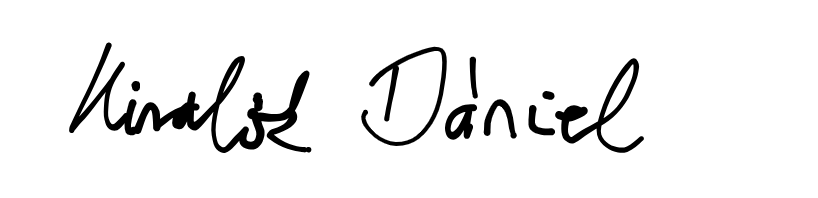
\includegraphics[width=175pt]{ alairas.png }}
\setlength{\headheight}{4em} 
\setlength{\parskip}{0.22em} 

\begin{document}
	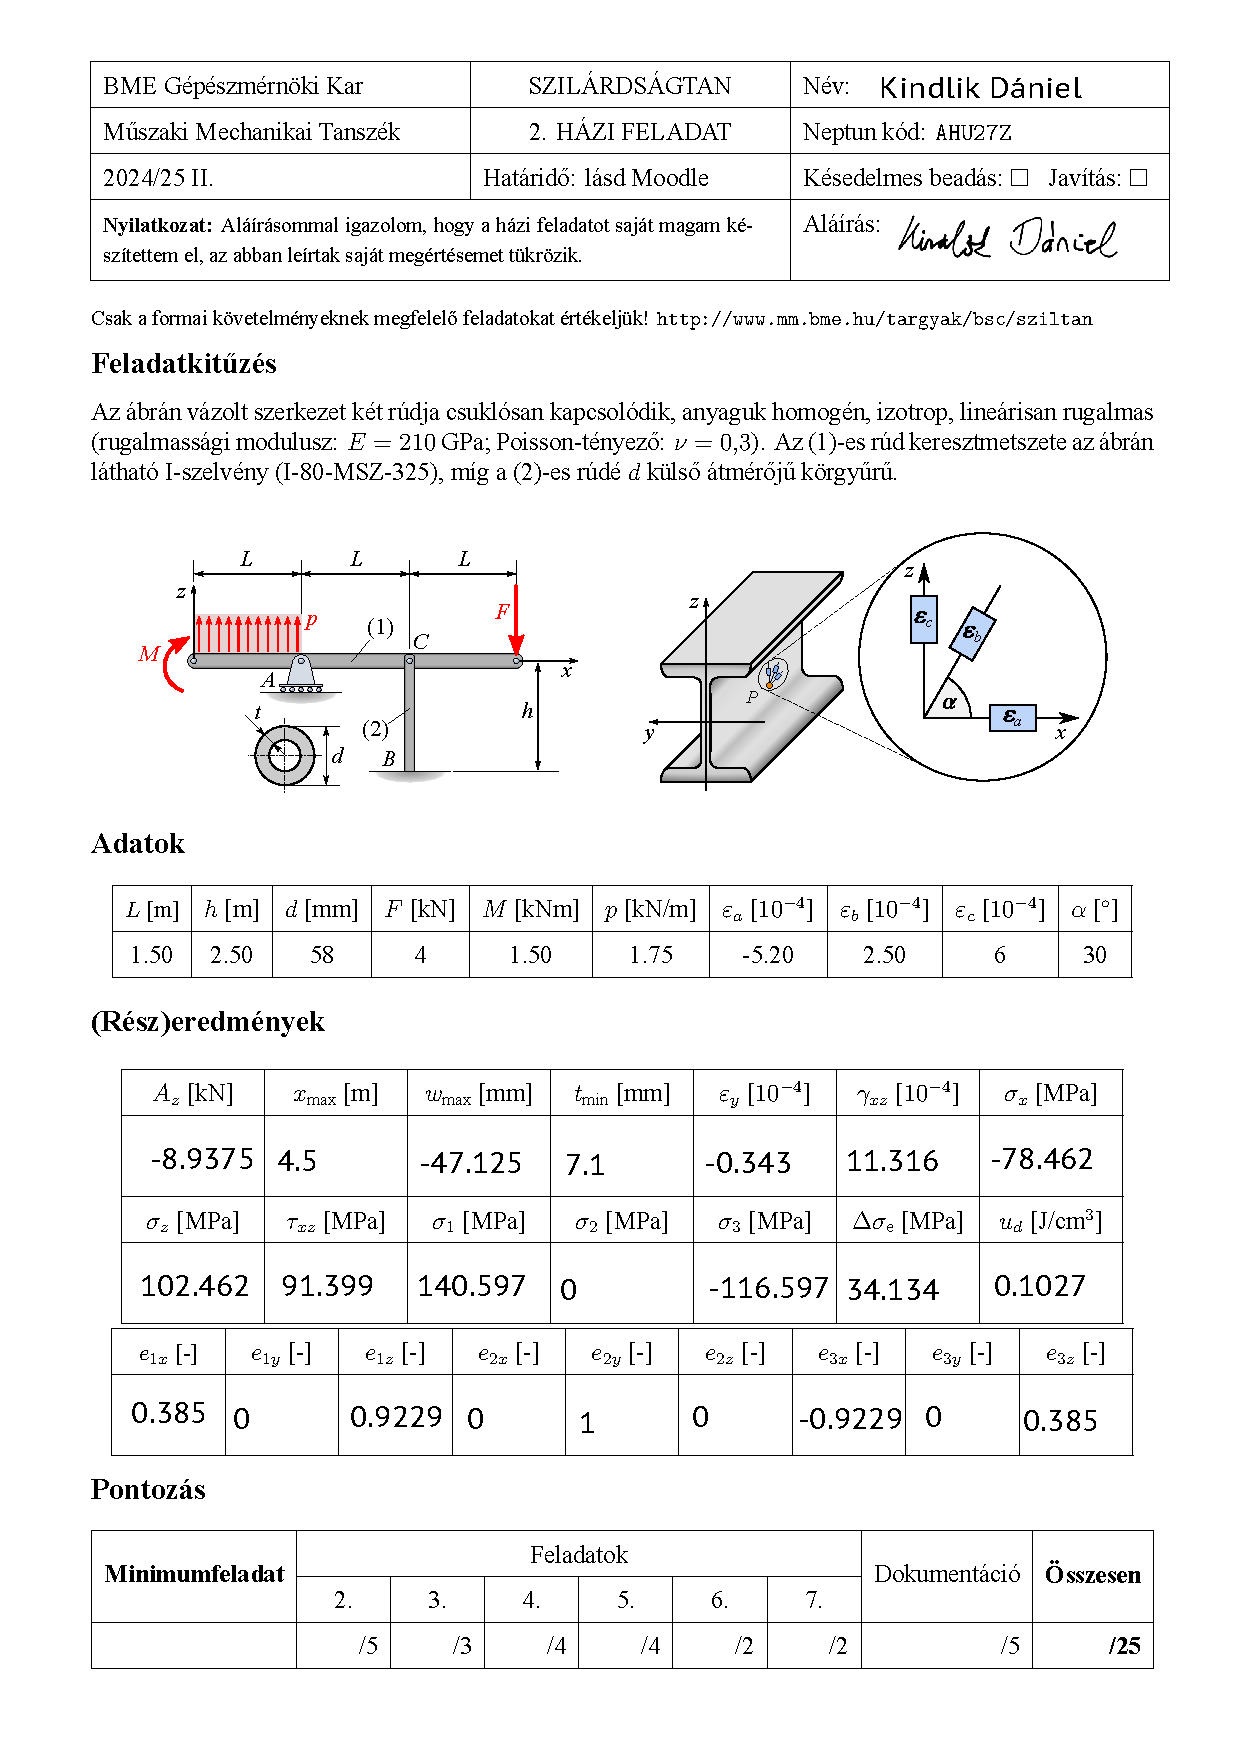
\includepdf[pages=1]{elolap.pdf}
	\adat
	$ L = 1.5\;\meter \;\;\;$ $ h = 2.5\;\meter \;\;\;$ $ d = 58\;\mm$\\\\
	$ F = 4\;\kn \;\;\; $ $ M = 1.5\knm $ $ p = 1.75\;\pknm \;\;\;$\\\\
	$ \epsilon_A = -5.2\;\minegy \;\;\;$ $ \epsilon_B = 2.5\;\minegy \;\;\;$ $ \epsilon_C = 6\;\minegy \;\;\;$ $ \alpha = 30\;\fok \;\;\;$\\\\
	$ E = 210\;\gpa \;\;\;$ $ \nu = 0.3\;\dimnel \;\;\;$
	\setcounter{page}{1}
	\egy
	\begin{center}
		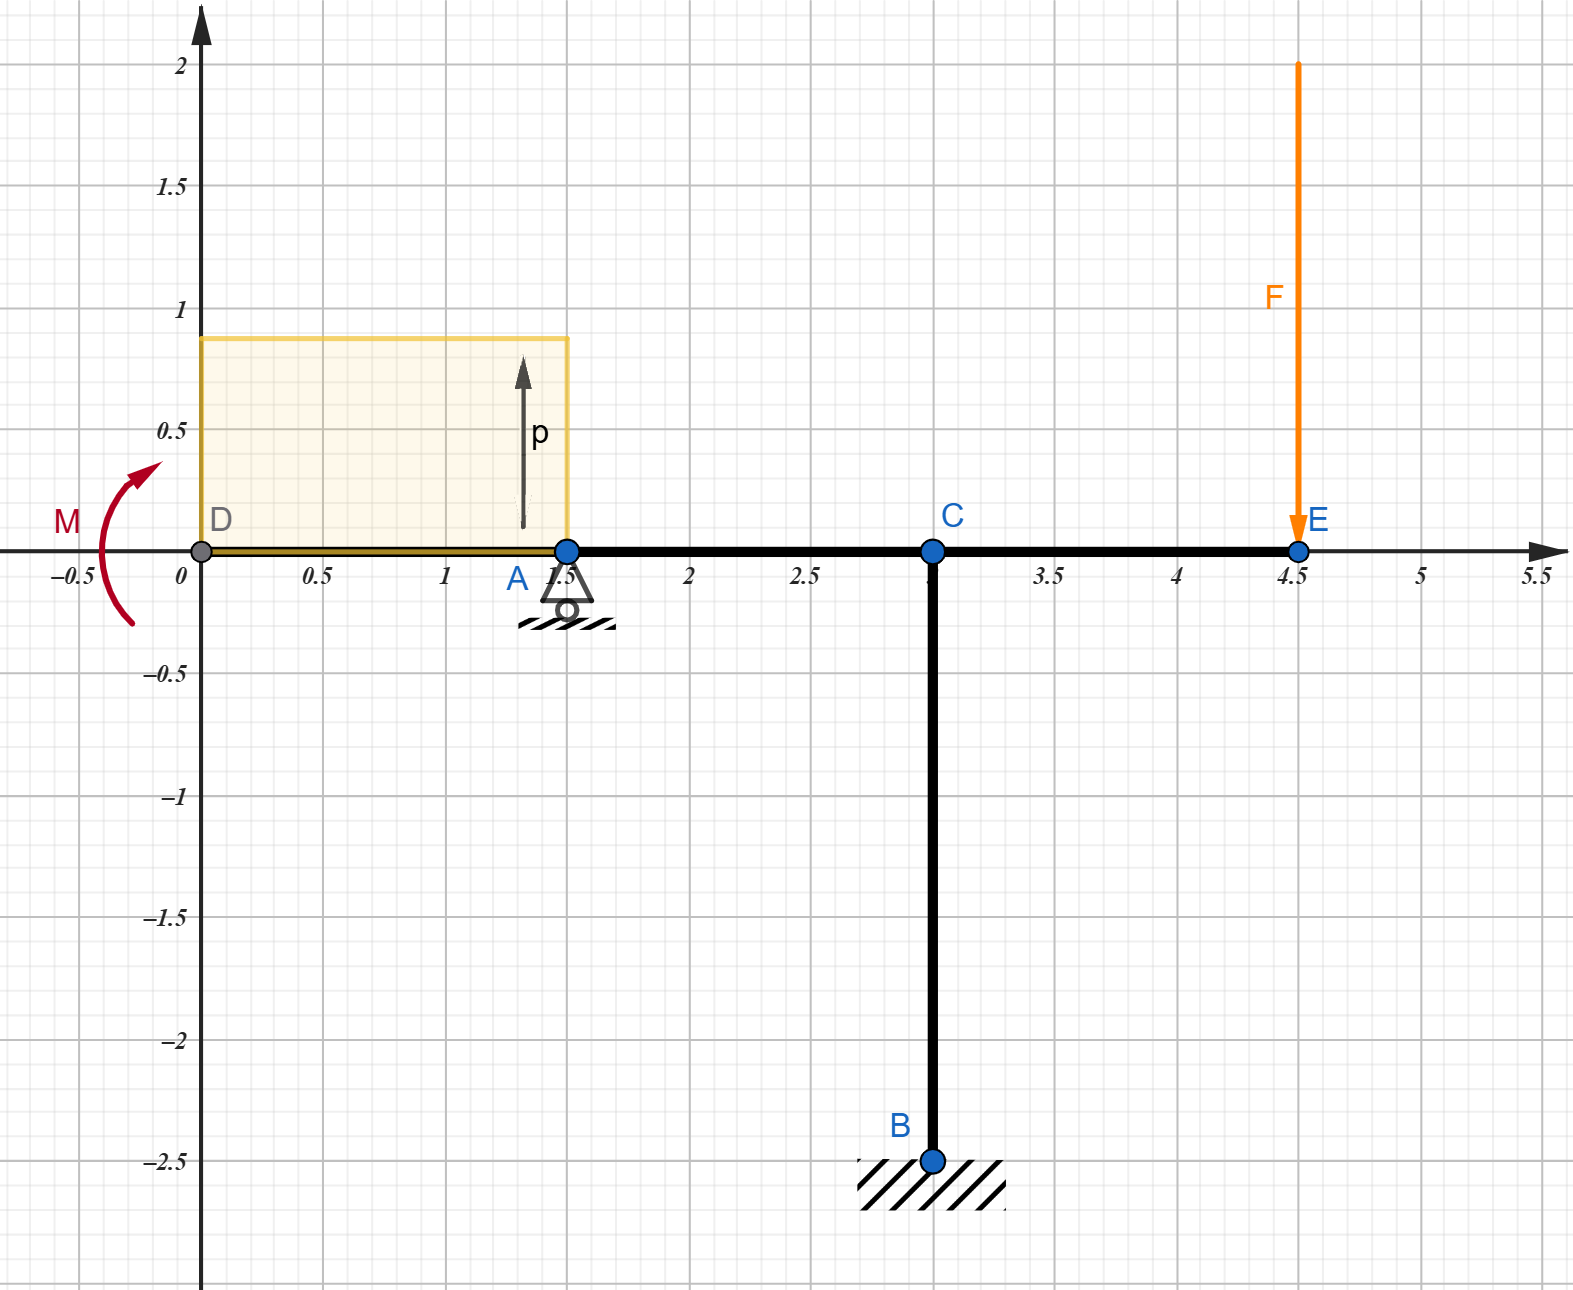
\includegraphics[width=200pt]{ meretarany.png }\\
		Az ábrán egy egység megfelel 1 m-nek és 2 kN-nak
	\end{center}
	A szerkezetünket két részre tudjuk bontani, hogy ki tudjuk számolni a reakcióerőket.\\
	Ekkor C-pontban meg fog jelenni egy C vektor, és a két rúdra külön tudunk 3-3 egyensúlyi-egyenletet írni.
	A két rész (1. eset balra, 2. eset jobbra) szabadtest-ábrája:
	\begin{center}
		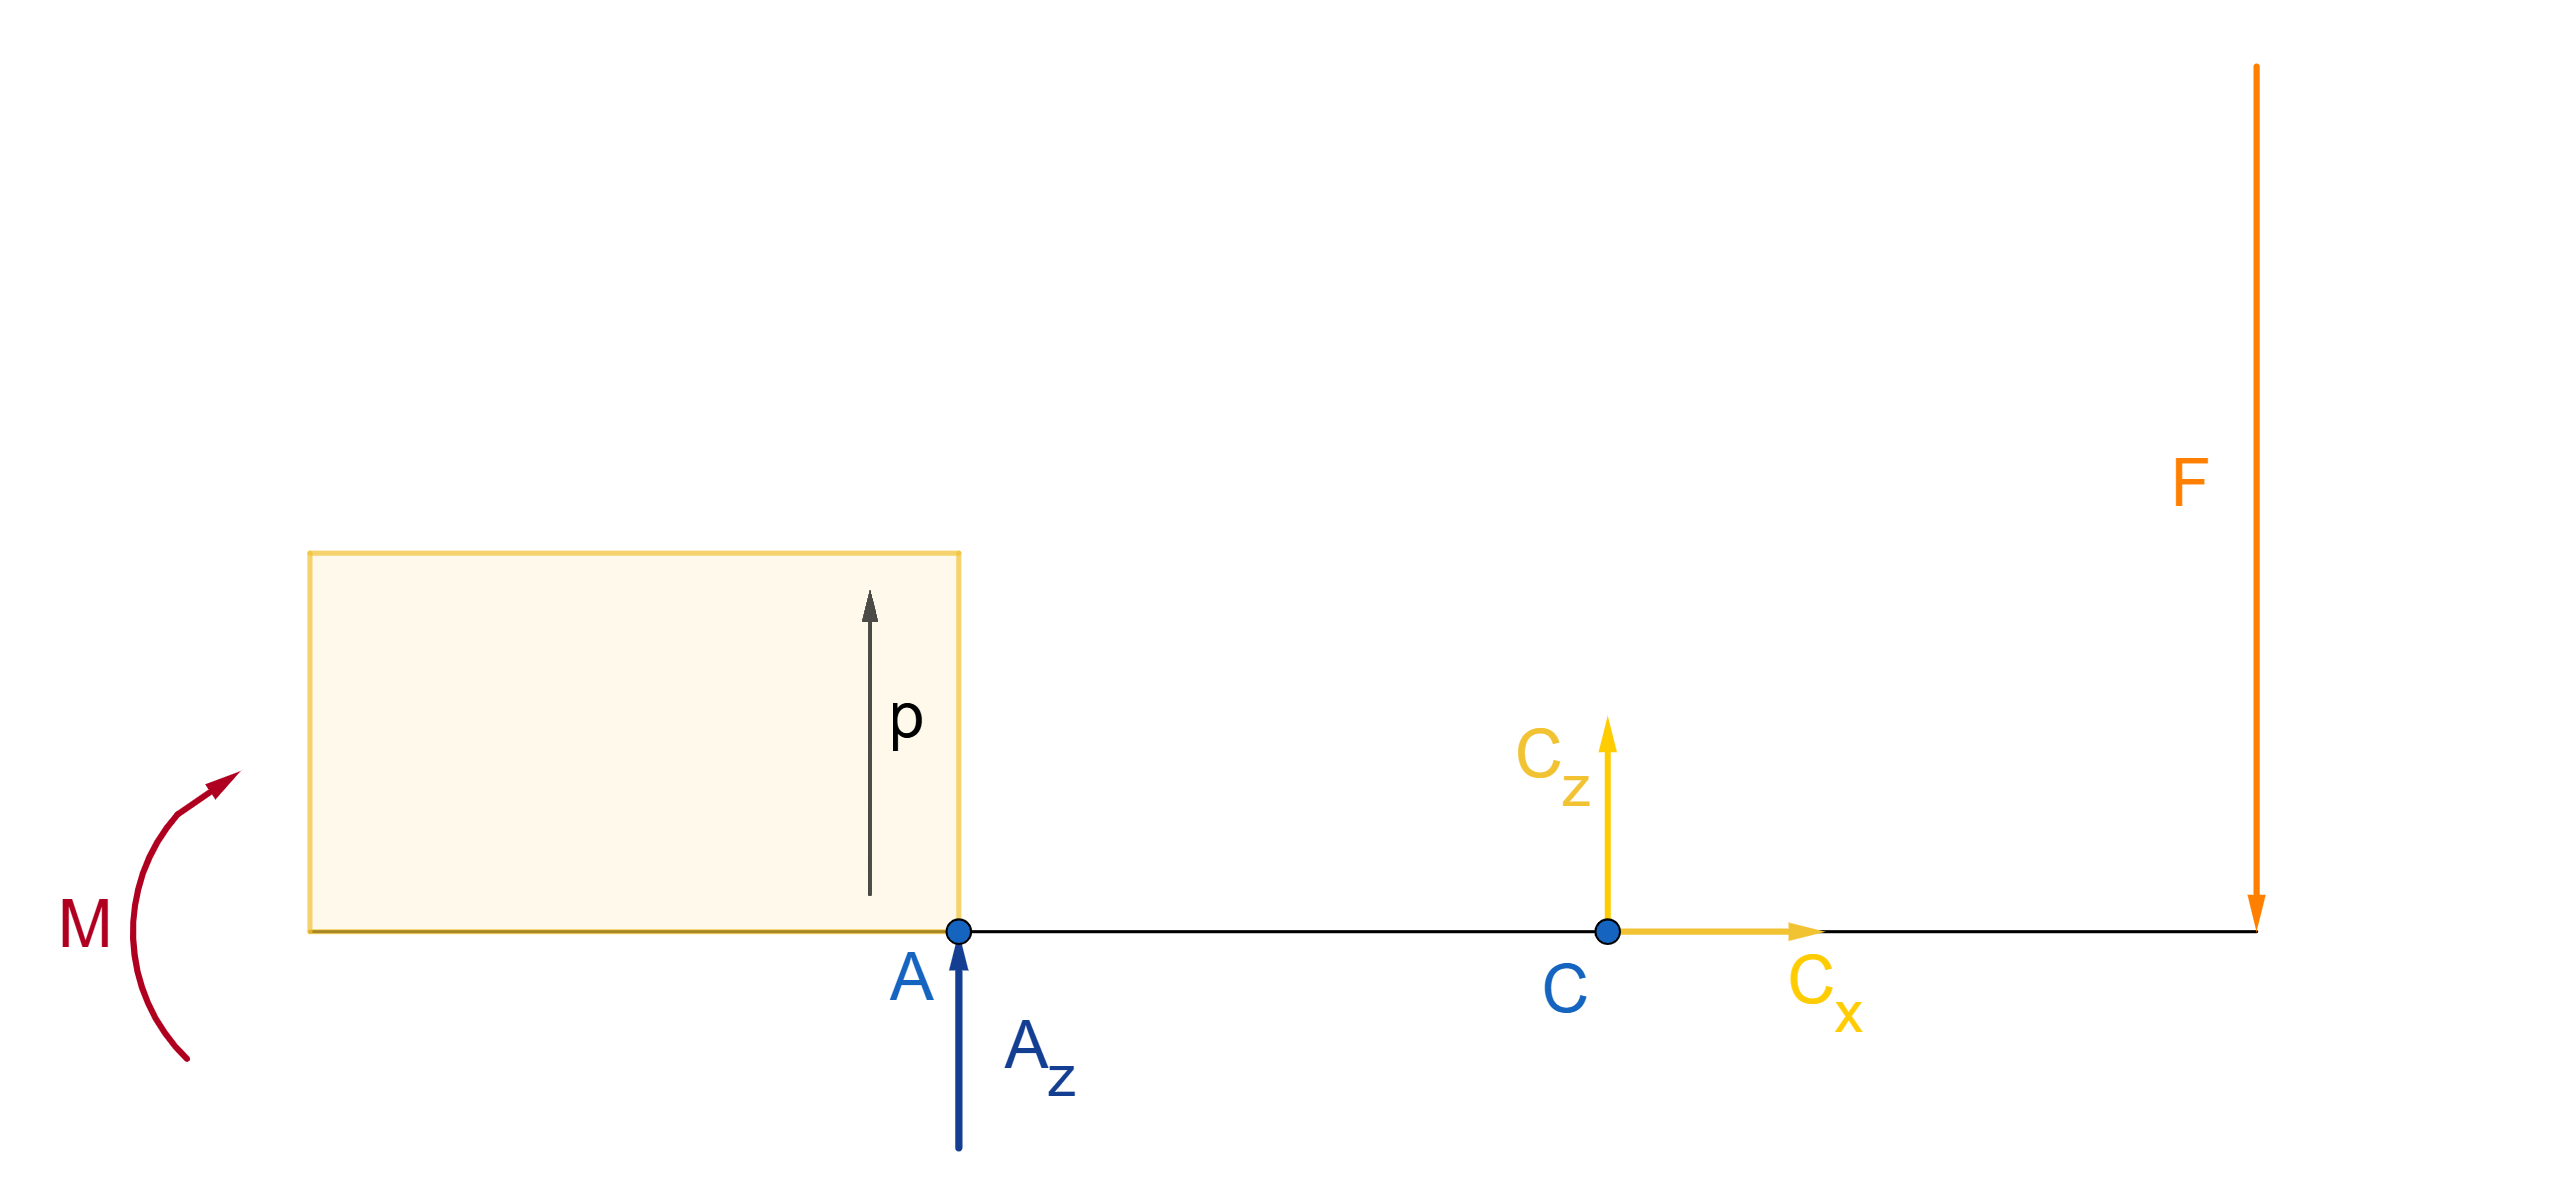
\includegraphics[width=270pt]{ SZTA1.png }
		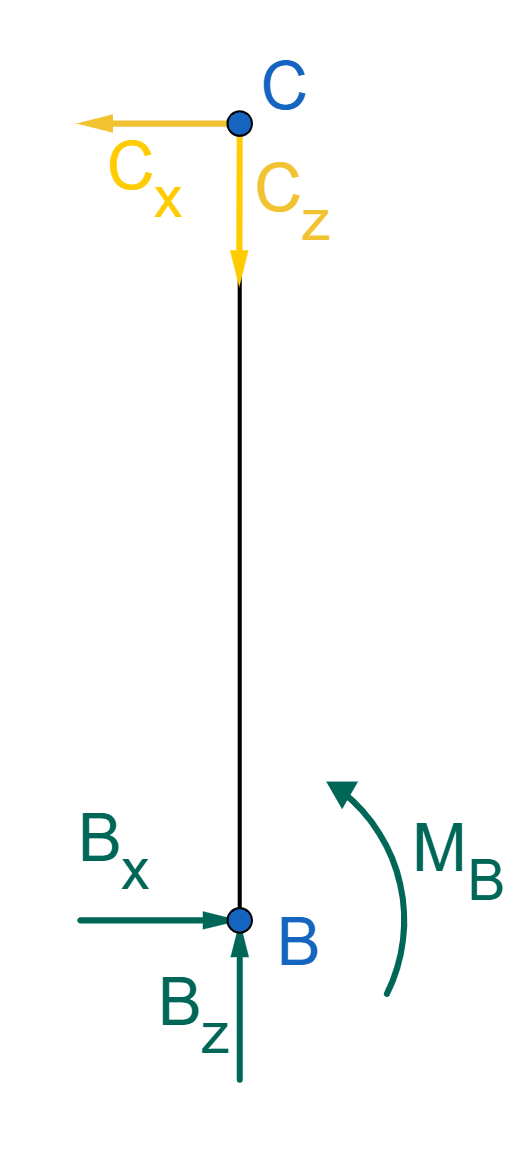
\includegraphics[width=70pt]{ SZTA2.png }
	\end{center}
	$ $\\\\\\\\
	1. esetben kijövő egyensúlyi egyenletek A pontra vonatkoztatva:\\\\
	\tabto{50pt}(1) $\sum{F_x} = 0 = C_x$\\\\
	\tabto{50pt}(2) $\sum{F_y} = 0 = A_z + C_z + p \cdot L - F$\\\\
	\tabto{50pt}(3) $\sum{M_{A'}} = 0 = C_z \cdot L - M - F \cdot 2L - (p \cdot L) \cdot \frac{L}{2}$\\\\
	2. esetben kijövő egyensúlyi egyenletek B pontra vonatkoztatva:\\\\
	\tabto{50pt}(4) $\sum{F_x} = 0 = -C_x + B_x$\\\\
	\tabto{50pt}(5) $\sum{F_y} = 0 = -C_z + B_z$\\\\
	\tabto{50pt}(6) $\sum{M_B} = 0 = M_B + B_x \cdot h$\\\\
	A két egyenletrendszer megoldása:\\\\
	\tabto{50pt}$A_z = \underline{\underline{-8.9375 \kn}}$\\\\
	\tabto{50pt}$B_x = \underline{\underline{0 \kn}}$\\\\
	\tabto{50pt}$B_z = \underline{\underline{10.3125 \kn}}$\\\\
	\tabto{50pt}$M_B = \underline{\underline{0 \kn}}$\\\\
	\tabto{50pt}$C_x = \underline{\underline{0 \kn}}$\\\\
	\tabto{50pt}$C_z = \underline{\underline{10.3125 \kn}}$
	\newpage
	\ketto
	Ahhoz hogy meg tudjuk határozni w(x)-et először meg kell adnunk az (1)-es rúd hajlítónyomatéki igénybevételét:
	A szerkezetet három részre tudjuk bontani, így a függvény:
	\begin{table}[h]
		\renewcommand{\arraystretch}{1.8}
		\resizebox{\textwidth}{!}{%
			\centering
			\begin{tabular}{c|c|c|c|c}
				& N                     & V                                                                                  & $\text{M}_\text{h}$                                                                                                                            & $\text{M}_\text{t}$ \\ \hline
				\begin{tabular}[c]{@{}c@{}}I.\\ $0 < x < 1$\end{tabular}   & $- A_x = 4 \kn$       & \begin{tabular}[c]{@{}c@{}}$A_y - x \cdot p =$\\ $= 7.5577 -5x \kn$\end{tabular}   & \begin{tabular}[c]{@{}c@{}}$M_A - x \cdot A_y + \dfrac{x}{2} \cdot (x \cdot p) =$\\ $= 2.5x^2 - 7.5577x + 5.8577 \knm$\end{tabular}            & $0 \knm$                 \\ \hline
				\begin{tabular}[c]{@{}c@{}}II.\\ $1 < x < 1.7$\end{tabular}  & $- A_x + C_x = 0 \kn$ & \begin{tabular}[c]{@{}c@{}}$A_y - x \cdot p =$\\ $= 7.5577 -5x \kn$\end{tabular}   & \begin{tabular}[c]{@{}c@{}}$M_A - M_C - x \cdot A_y + \dfrac{x}{2} \cdot (x \cdot p) =$\\ $= 2.5x^2 - 7.5577x + 5.0577 \knm$\end{tabular}      & $0 \knm$                 \\ \hline
				\begin{tabular}[c]{@{}c@{}}III.\\ $1.7 < x < 2.3$\end{tabular} & $- A_x + C_x = 0 \kn$ & \begin{tabular}[c]{@{}c@{}}$A_y - (a + b) \cdot p=$\\ $= -0.9423 \kn$\end{tabular} & \begin{tabular}[c]{@{}c@{}}$M_A - M_C - x \cdot A_y + (x - \dfrac{a + b}{2}) \cdot ((a + b) \cdot p) =$\\ $= 0.9423x - 2.1673 \knm$\end{tabular} & $0 \knm$                 \\
			\end{tabular}%
		}
	\end{table}
\end{document}